\section{Evaluation}
\label{sec:eval}

We have implemented our technique for repairing type errors for a purely
functional subset of \ocaml with polymorphic types and functions. We seek to
answer the following Research Questions:

\begin{itemize}
    %%% FIXME: only some initial thoughts
    \item \textbf{RQ1}: What is the \emph{quality} of \toolname's repairs?
    \item \textbf{RQ2}: Does \toolname correctly \emph{localize} errors?
    \item \textbf{RQ3}: Do our ML models \emph{generalize} well for error
    localization and template prediction?
    \item \textbf{RQ4}: Are \toolname's repairs actually useful to novice programmers
    for feedback generation?
\end{itemize}

We first present our experimental methodology and then we will try to answer
each of the above questions, drawing from our results from a human study and our
manual evaluation.


\subsection{General Methodology}
\label{subsec:gen_method}
To answer our questions, we use an \ocaml dataset gathered from an
undergraduate Programming Languages course at UNKNOWN UNIVERSITY, previously
used in related work [FIXME: cite]. This dataset consists of ill-typed programs
and their subsequent fixes, drawn from two different years of that class, The
first part of the dataset comes from the Spring 2014 class (\SPRING), with a
cohort of 46 students and the second comes from the Fall 2015 class (\FALL),
with a cohort of 56 students. This homework require students to write 23
distinct programs. While the extracted programs are relatively
small, they demonstrate a range of functional programming idioms, \eg
higher-order functions and (polymorphic) algebraic data types.

\mypara{Feature Extraction}
We extract 416 features from each sub-expression in a
program, including:
%
\begin{enumerate}
  \item 45 local syntactic features.
  \item 315 contextual syntactic features. For each sub-expression we
    additionally extract the local syntactic features of its first, second,
    third and fourth (left-to-right) children. In addition, we extract those
    features for its ancestors, starting from its parent and going up to two
    more parent nodes. If an expression does not have a ancestor or children,
    these features will simply be disabled. If an expression has more than four
    children, the classifiers will receive no information about the additional
    children.
  \item 88 typing features. We support |int|s, |float|s, |char|s, |string|s, and
    the user-defined |expr|. These features are extracted for each
    sub-expression and its context.
  \item 1 feature denoting the size of each sub-expression.
\end{enumerate}

\mypara{Dataset ``cleaning''}
We automatically extract a blame oracle for each ill-typed program from the
(AST) diff between it and the student's eventual fix. A disadvantage of using
diffs in this manner is that students may have made many, potentially unrelated,
changes between compilations; at some point the ``fix'' becomes a ``rewrite''.
We do not wish to consider the ``rewrites'' in our evaluation, so we discard
outliers where the fraction of expressions that have changed is more than one
standard deviation above the mean, establishing a diff threshold of 40\%. We
also discard programs that changed in 5 or more locations, since we consider
these to also be ``rewrites''. It
is also highly unlikely that such ``fixes'' can reproduced by \toolname or any
related work [FIXME: cite relevant]. All these discarded outliers account for
roughly 32\% of each dataset, leaving us with 2,475 program pairs for \SPRING
and 2,177 pairs for \FALL. For all of our tests, we use \SPRING as a training
set and \FALL as a test set.

\mypara{Accuracy Metrics}
A recent study of fault localization techniques \citep[][]{Kochhar2016-oc} shows
that most developers will not consider more than around five potential error
locations before falling back to manual debugging. We evaluate \toolname's
location predictions of possible errors, considering if the user's changes
occurred in our top three or top five predictions, but our automatic method of
producing fixes may consider more than that. We also extend such intuition, that
a user won't consider more than five ``suggestions'' as feedback, to possible
fixes, and thus we evaluate \toolname's top six template predictions on whether
they include the correct template, \ie the one that matches the user's change. We also
include the confusion matrix of the top-one predictions for all locations, in
order to present what templates our models usually mix together and see if they
generalize well between different groups of solutions.

\mypara{Repair Quality}
Finally, for a more qualitative evaluation of \toolname's synthesized solutions
based on the above results, we ran a human study at UNKNOWN UNIVERSITIES. Each
participant was asked to evaluate the quality of the program fixes and their
locations against \seminal's repairs \citep{Lerner2006-pj, Lerner2007-dt}. For
each program, beside the two repairs, the participants were given the original
ill-typed program, along with the standard \ocaml compiler's error message and a
short description of what the original author of the program intended it to do.

\subsection{Quantitative Evaluation}
\label{subsec:quan_eval}

First, we evaluate the accuracy of our predictions for both type error
localization and template prediction.


\subsubsection{Template Prediction Accuracy}
\label{subsubsec:templ_acc}

\mypara{Baselines}
We provide two baselines for the comparison: a random choice of template and a
prediction based on popularity.

\mypara{Our Classifiers}
We evaluate our classifiers, each trained on the \SPRING quarter and evaluated
on the \FALL quarter. These include:
\begin{description}
  \item[\random] A dummy classifier that \emph{uniformly} selects each time a
    template to return. There is no training necessary with this classifier.
  \item[\popular] This classifier returns always the most popular template from
    the training set. As a second prediction returns the second most popular
    template and so on. The training phase of this classifier includes just
    learning the popularity of each cluster-template on the training set.
  \item[\textsc{Deep Neural Network} (\dnn)] A multi-layer perceptron neural
    network, trained with $\eta = 0.001$, $\lambda = 0.001$, and a mini-batch
    size of 256. Our network utilizes three fully-connected hidden layers of 512
    neurons. The neurons use rectified linear units (ReLU) as their activation
    function, a common practice in modern neural networks.
\end{description}

All classifiers were trained using the \emph{early stopping} approach, where the
training of a neural network is stopped when the accuracy on a distinct small
part of the training set is not improved after a certain amount of epochs. We
set that amount to 5 and the maximum number of epochs to 200. The \textsc{Adam}
optimizer \citep{Kingma2014-ng}, a variant of stochastic gradient descent that
has been found to converge faster, was used to train our \dnn.

% colors from http://colorbrewer2.org/?type=sequential&scheme=Blues&n=3
\definecolor{blue1}{HTML}{DEEBF7}
\definecolor{blue2}{HTML}{9ECAE1}
\definecolor{blue3}{HTML}{3182BD}
\definecolor{green1}{HTML}{E5F5E0}
\definecolor{green2}{HTML}{A1D99B}
\definecolor{green3}{HTML}{31A354}

\begin{figure}[t]
\centering
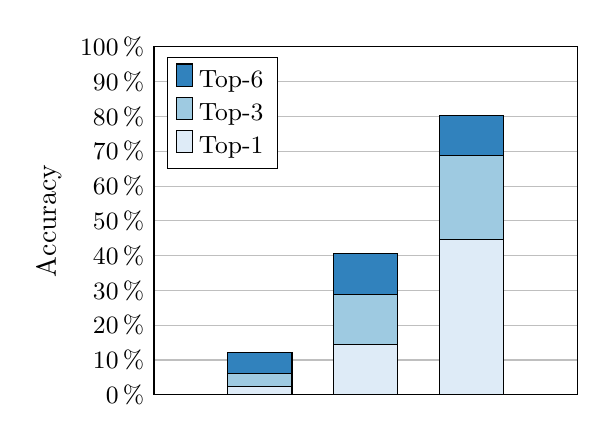
\begin{tikzpicture}
\begin{axis}[
  ybar stacked,
  % width=\linewidth,
  height=6cm,
  % title={Accuracy of Repair Template Prediction},
  ylabel={Accuracy},
  bar width=0.82cm,
  ymin=0.0,
  ymax=100.0,
  ytick={0.0, 10.0, 20.0, 30.0, 40.0, 50.0, 60.0, 70.0, 80.0, 90.0, 100.0},
  yticklabel={\pgfmathparse{\tick}\pgfmathprintnumber{\pgfmathresult}\,\%},
  ytick style={draw=none},
  ymajorgrids = true,
  symbolic x coords={random, popular, dnn},
  enlarge x limits=0.5,
  xtick=data,
  xtick style={draw=none},
  xticklabels={\random, \popular, \dnn},
  %x tick label style={rotate=45, anchor=north east},
  x tick label style={font=\small},
  y tick label style={font=\small},
  reverse legend,
  transpose legend,
  legend style={legend pos = north west, legend columns=4, font=\small},
]

\addplot[draw=black, fill=blue1] coordinates {(random, 2.35646958011996552) (popular, 14.438731790916881) (dnn, 44.64438731790917)};
\addlegendentry{Top-1}
\addplot[draw=black, fill=blue2] coordinates {(random, 3.6846615252784924) (popular, 14.395886889460153) (dnn, 24.250214224507282)};
\addlegendentry{Top-3}
\addplot[draw=black, fill=blue3] coordinates {(random, 6.212510711225363) (popular, 11.825192802056556) (dnn, 11.482433590402735)};
\addlegendentry{Top-6}

\end{axis}
\end{tikzpicture}
\caption{
  Results of our template prediction classifiers using the \emph{50 most
  popular} templates. We present the results up to the top 6 predictions, since
  our synthesis algorithm considers that many templates before falling to a
  different location.
}
\label{fig:accuracy-results}
\end{figure}


\begin{figure}[t]
  \centering
  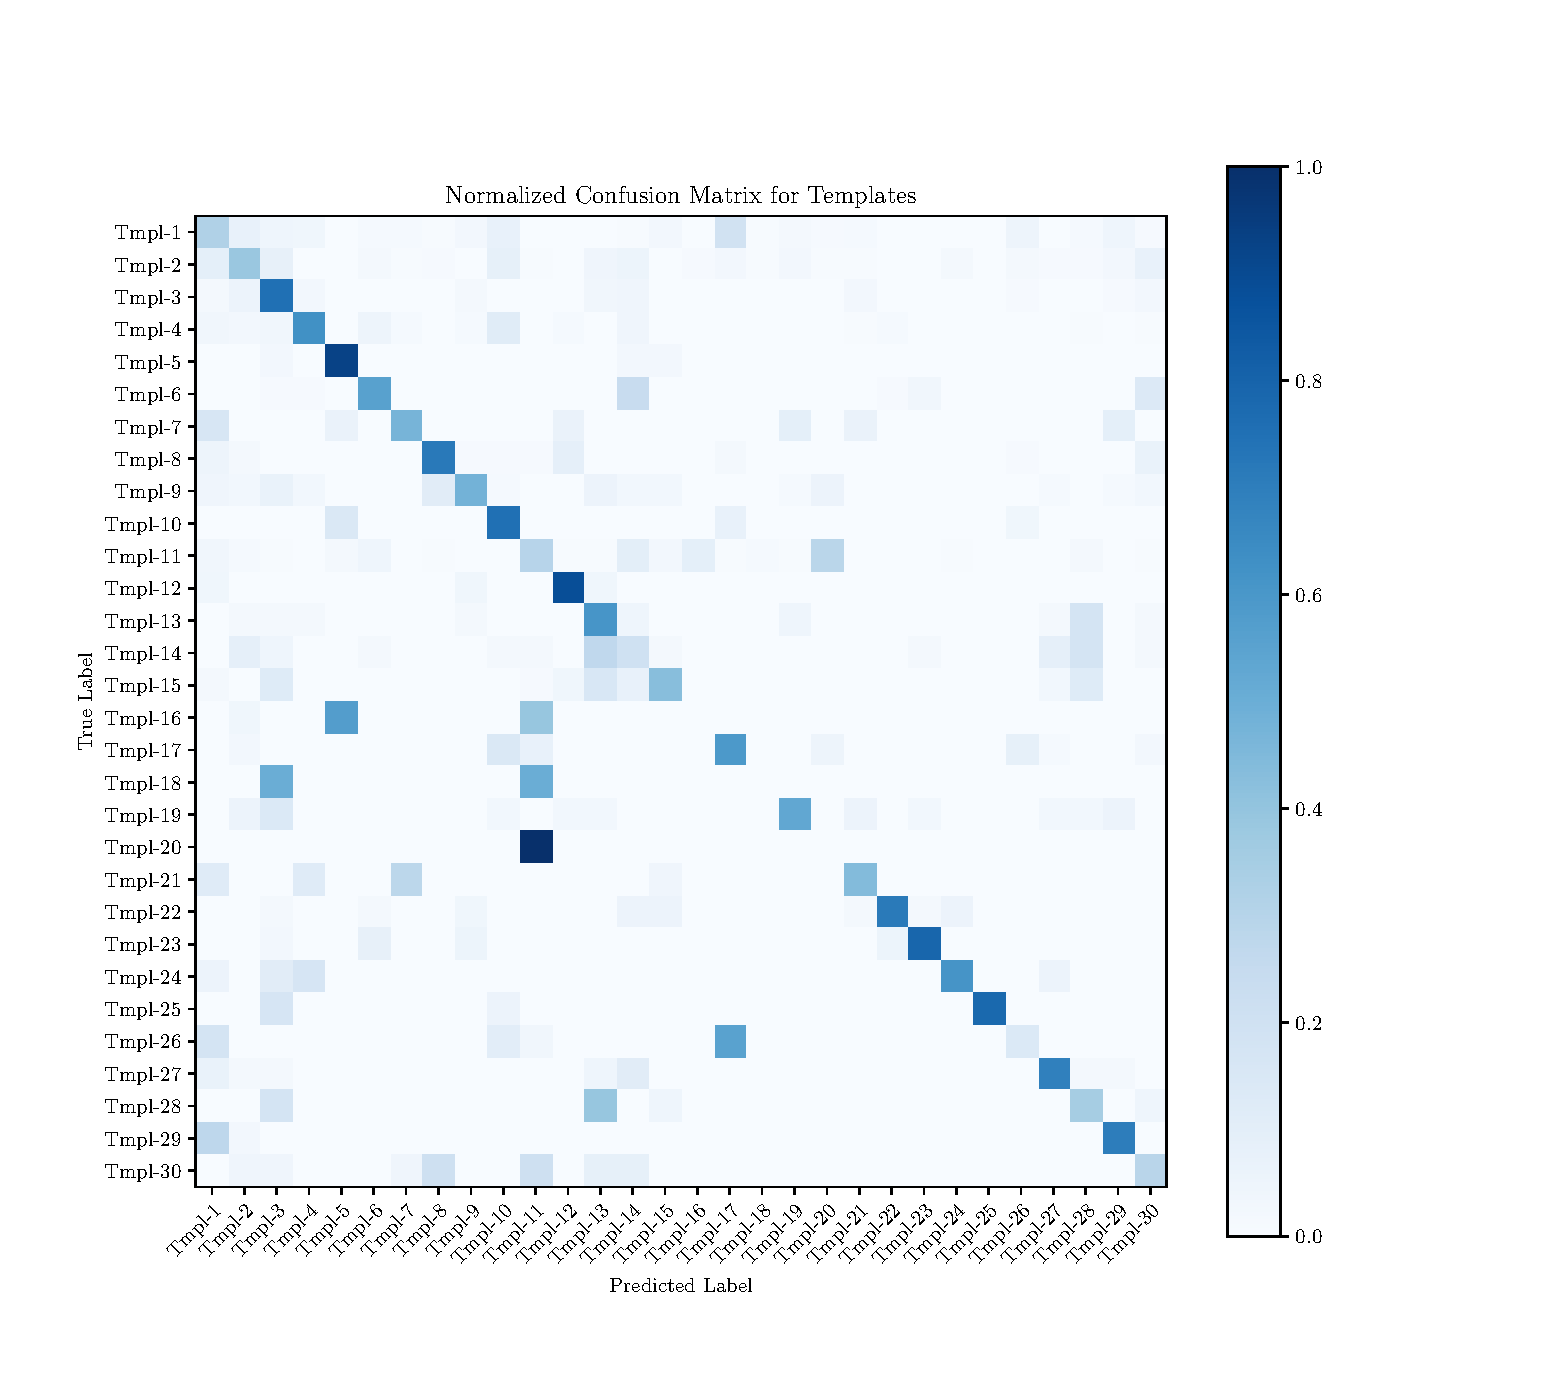
\includegraphics[trim={30 40 100 70},clip,width=\linewidth]{evaluation-conf-matrix.pdf}
  \caption{The confusion matrix of the \emph{top 30} templates. Bolder parts of
  the heatmap show templates that are often mis-predicted with another template.
  The bolder the diagonal values are, the more correct predictions we have.}
  \label{fig:conf-matrix}
\end{figure}

\mypara{Results}
\autoref{fig:accuracy-results} shows the accuracy results of our template
prediction experiments. The naive baseline of selecting templates at random
achieves \RandomTopOne\% Top-1 accuracy (\RandomTopSix\% Top-6), while the
\popular classifier achieves a Top-1 accuracy of \PopularTopOne\%
(\PopularTopSix\% Top-6). Our \dnn classifier significantly outperforms those naive
classifiers, ranging from \DnnTopOne\% Top-1 accuracy to \DnnTopSix\% Top-6
accuracy. Interestingly, with only \dnn's first prediction, one outperforms top
6 predictions of both \random and \popular.

The \random classifier selects \emph{randomly} a template, out of the 50 learned
ones from the \SPRING training dataset, for each location it is presented. It
was expected, therefore, to achieve such low accuracy, even for Top-6.
Surprisingly, the \popular accuracy results are not that low. This mainly
happens because of the nature of our dataset. Some homework assignments were
shared between \SPRING and \FALL quarters and, while different groups of
students solved these problems for each quarter, the novice mistakes that they
made seem to have a \emph{pattern}. Thus, the most \emph{popular ``fixes''} (and
therefore the relevant templates) that were applied to \SPRING, are also popular
in \FALL. However, the almost \emph{2x higher} accuracy of our \dnn classifier,
shows that we can learn a \emph{better pattern} from these datasets and that our
\dnn model is able to \emph{generalize} between different solutions of the
problems.

\autoref{fig:conf-matrix} further proves that our \dnn generalizes well. This
Figure includes the confusion matrix of the top 30 templates that were acquired
from the training set and were tested on the same \FALL dataset as before. We
observe that most of the templates are predicted correctly and only a few of
them are often mis-predicted for another template. For example, we see that
programs that would require template 20 to be fixed almost always are
mis-predicted with template 11. [TODO: show those two templates, both ``let''s
with some ``tuple'' in their ASTs]

\subsubsection{Error Localization Accuracy}
\label{subsubsec:error_loc_acc}

\mypara{Method}
For our error localization task, we again train a multi-layer perceptron neural
network, with the same hyper-parameters as in \ref{subsubsec:error_loc_acc}. Our
network firstly uses two fully-connected hidden layers of 1024 neurons and one
of 512 neurons before the output layer. The neurons again use rectified linear
units (ReLU) as their activation function and are trained using the \emph{early
stopping} approach and the \textsc{Adam} optimizer.

Previous work \citep[][]{Seidel:2017} has used more shallow neural networks, but
also fewer features per node. In our implementation, we added more contextual
features following recent research direction, which has shown them to be the
most important \citep[TODO: add the lstm paper][]{Seidel:2017}. Thus, we
chose deeper neural network architectures for our error localization models as
well.

\begin{table}
  \centering
  \begin{tabular}{l|rr}
    Classifier & Top-3  & Top-5 \\
    \hline
    \random   & 39.70\% & 58.73\% \\
    \toolname & 79.71\% & 88.83\% \\
  \end{tabular}
  \caption{Experimental results of \toolname's error localization accuracy.}
  \label{tab:err_loc_acc}
\end{table}

\subsubsection{Empirical Repair Quality Evaluation}
\label{subsubsec:man_rep_qual_eval}

\mypara{Synthesis Algorithm}
We guide our synthesis algorithm, using the above predictions for finding the
proper locations to fix and what template to use. Every program has a timeout of
\emph{30s} to be repaired by the synthesis algorithm. We observe that
\textbf{12.54\%} of our testing dataset's programs fail to be repaired within
that amount of time. The main reason is the combined failure of our
models to give high confidence to the correct locations and templates, thus
making the search very expensive. However, for the 87.46\% of the programs that
actually finish synthesizing, around \textbf{96.32\%} return a solution that
type-checks. The small amount of programs that couldn't find a well-typed
solution but still finished, usually required some bigger changes (\ie
expressions whose ASTs were deeper than 4 levels) that our algorithm didn't
explore in this version.

Finally, all these solutions that did not timeout, had an average time of
synthesis of \textbf{9.26s}. From the well-typed solutions that we got, almost
\textbf{11\%} of them give the exact same repair as the user did, in any of the
suggested top 3 repairs. While that amount seems small, it is a considerable
amount in the correct direction meaning that our models can learn novice's
intents in bug fixing.

%%% TODO: Maybe self-evaluate 50-100 synthesized programs?

\subsection{Qualitative Evaluation}
\label{subsec:quan_eval}

To assess the quality of \toolname's repairs, we conducted an IRB-approved human
study with 28 participants. From this study, we found that both the edit
locations and final repairs produced by \toolname were better than those
produced by \seminal (FIXME cite), a state of the art Ocmal repair tool, in a
statistically significant manner. Subsection~\ref{subsubsec:study_setup}
describes our experimental design, and subsection~\ref{subsubsec:study_res}
presents our detailed findings.

\subsubsection{Human Study Setup}
\label{subsubsec:study_setup}

% FIXME? Add some intro sentence here?

For our human study, participants were recruited from \emph{two public research
institutes removed for blind review}. The study was also advertised on twitter.
To be included for analysis, participants had to assess the quality and give
comprehensible bug descriptions of at least 5 / 10 stimuli. In total, there were
28 valid participants, and the study took around 25 minutes to complete. For
compensation, participants had the option to enter a drawing for an Amazon Echo
voice assistant.

To create the stimuli, a corpus of 21 buggy programs were randomly selected from
1834 type-correct synthesized programs. From this corpus, each participant was
then shown 10 randomly selected programs. Along with each buggy program,
participants were also shown two candidate repairs: one generated by \toolname
and one by \seminal. For both, we used the highest-ranked solution that they
returned. The participant was always unaware which tool generated which
candidate patch. Participants were then asked to assess the quality of each
candidate repair on a Likert scale of 1 to 5. They were further asked for a
binary assessment of the quality of each repair's edit location. An example
stimulus can be found in \autoref{fig:stimulus}.

In our study, we also collected self-reported estimates of both programming and
\ocaml-specific experience as well as qualitative data assessing factors
influencing each participant's subjective judgment of repair quality.

\begin{figure}
  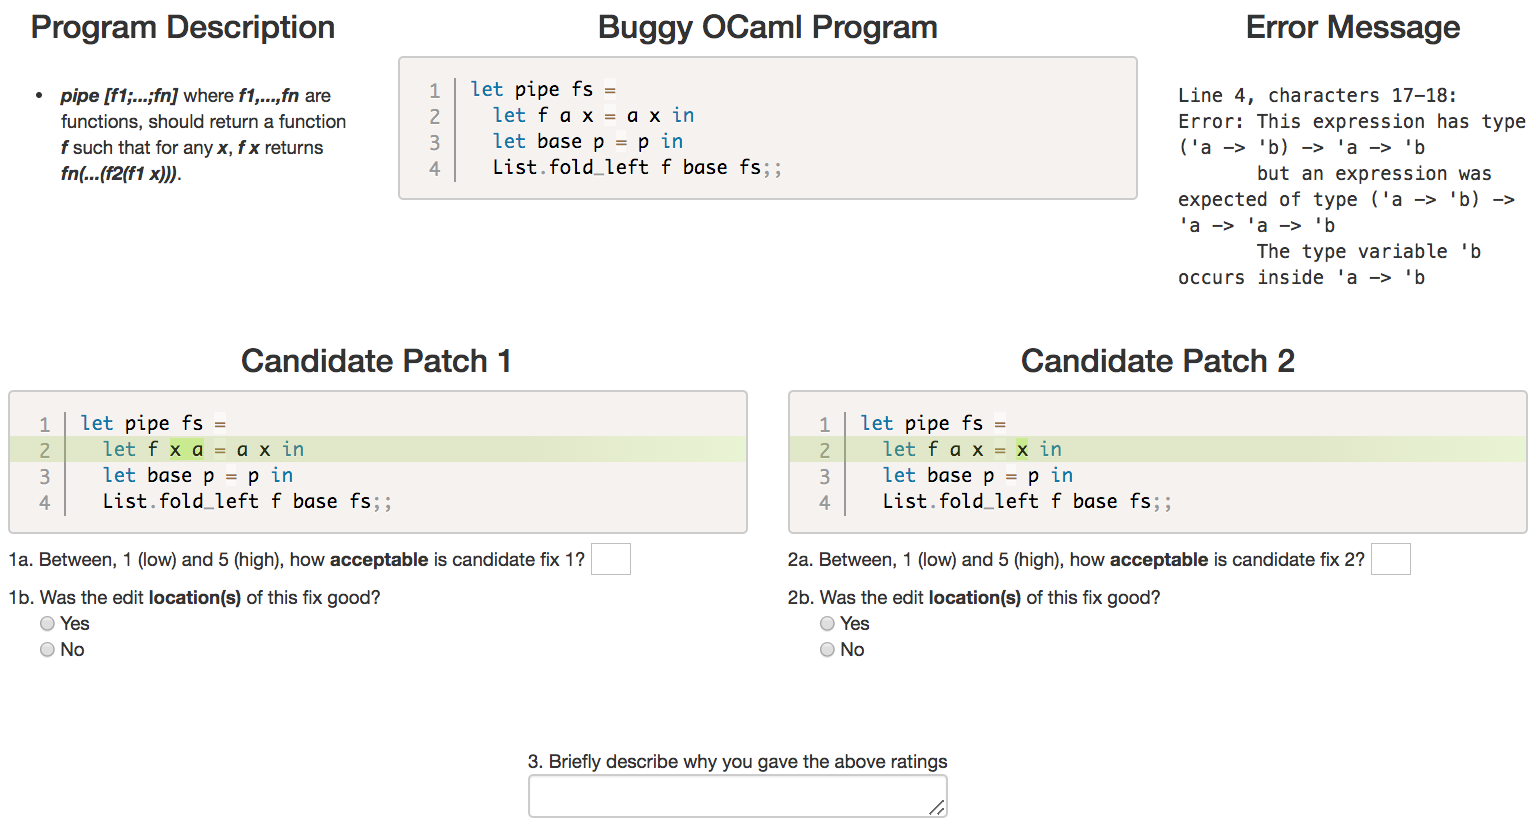
\includegraphics[width=8cm]{SampleStimuli.png}
  \caption{A sample stimulus used for assessing repair quality.}
  \label{fig:stimulus}
\end{figure}

\subsubsection{Human Study Results}
\label{subsubsec:study_res}

% FIXME: Intro sentence here.

From the 28 participants, we collected 534 patch quality assessments, 267 each
for \toolname and \seminal generated repairs. Overall, we found that \toolname's
repairs are 115.3\% the quality of \seminal's repairs ($p=0.022$). Specifically,
\toolname's repairs achieved an average quality rating of 2.41/5 while
\seminal's repairs had an average rating of only 2.09/5. All tests for
statistical significance used the Wilcoxon signed-rank test.

To tease apart this quality assessment, we also asked participants to assess
just the quality of the repair's edit location rather than the final repair.
From this data, we found that \toolname identified a viable edit location 81.3\%
of the time while \seminal only found a good edit location 73.0\% of the time.
Our participants, therefore, perceived \toolname's fault localization accuracy
as 10\% better than \seminal's. This difference was statistically significant
($p=0.018$).

% FIXME: Maybe add a paragraph here on qualitative results

Together, these two results demonstrate that humans perceive \toolname's repair
quality to be significantly better than the current state of the art, both in
terms of edit location accuracy and the quality of the overall repair.
